%% ============================================================
%%  LMBayes Meeting 2026 — Discussion Handout
%%  Adjective Ordering Preferences: An Incremental RSA Account
%%  Draft  |  \today
%% ============================================================
\documentclass[11pt, a4paper]{article}

% ---- packages ---------------------------------------------------------------
\usepackage[T1]{fontenc}
\usepackage[utf8]{inputenc}
\usepackage[margin=2.2cm]{geometry}
\usepackage{microtype}
\usepackage{booktabs}
\usepackage{tabularx}
\usepackage{multirow}
\usepackage{amsmath, amssymb}
\usepackage{mathtools}
\usepackage{bm}
\usepackage{graphicx}
\usepackage[dvipsnames]{xcolor}
\usepackage{enumitem}
\usepackage{parskip}          % paragraph spacing instead of indent
\usepackage{natbib}
\usepackage{hyperref}
\hypersetup{
  colorlinks = true,
  linkcolor  = MidnightBlue,
  citecolor  = MidnightBlue,
  urlcolor   = MidnightBlue,
}
\usepackage{cleveref}
\usepackage{tcolorbox}
\tcbuselibrary{breakable, skins}

% ---- convenience commands ---------------------------------------------------
\newcommand{\eg}{\textit{e.g.}}
\newcommand{\ie}{\textit{i.e.}}
\newcommand{\cf}{\textit{cf.}}
\newcommand{\adj}[1]{\textsc{#1}}   % adjective categories: \adj{D}, \adj{C}
\newcommand{\utter}[1]{\textsf{#1}} % utterances: \utter{DC}
\newcommand{\param}[1]{\ensuremath{#1}}
\newcommand{\todo}[1]{\textcolor{BrickRed}{\textbf{[TODO: #1]}}}

% ---- coloured discussion boxes ----------------------------------------------
\newtcolorbox{discussbox}[1]{
  colback  = gray!8,
  colframe = MidnightBlue!60,
  title    = {Discussion: #1},
  fonttitle= \bfseries\small,
  breakable
}
\newtcolorbox{resbox}[1]{
  colback  = green!5,
  colframe = OliveGreen!60,
  title    = {Key Result: #1},
  fonttitle= \bfseries\small,
  breakable
}

% ---- title ------------------------------------------------------------------
\title{
  \textbf{Adjective Ordering Preferences: \\
  An Incremental RSA Account with Bayesian Inference}\\[6pt]
  \large LMBayes Meeting 2026 --- Discussion Handout
}
\author{Hening Wang \quad Fabian Schlotterbeck \& \quad Michael Franke}
\date{\today \quad (Toward (finally!!)a first draft)}

% =============================================================================
\begin{document}
\maketitle
\tableofcontents
\bigskip

% =============================================================================
\section*{Introduction}
\label{sec:intro}
% =============================================================================

Speakers of diverse languages exhibit robust ordering preferences of adjectives (e.g., preferring “the big brown bag” over “the brown big bag”).
A way to approach this regularity is through communicative efficiency: helping interlocutors coordinate quickly and reliably. Yet “efficiency” can be formalized from two perspectives that make different ordering predictions: a hierarchical, comprehension-oriented view in which modification is composed outward from the noun, and a linear, production-oriented view in which speakers benefit from placing highly informative material early in the unfolding word stream. 
The present project pursues a third, unified perspective: adjective ordering
explained by \emph{incremental pragmatic reasoning}, where a speaker produces
one adjective at a time and the in-context informativeness of each adjective
interacts with its inherent semantic precision.

The project has three interlocking components:
\begin{enumerate}[label=\arabic*.]
  \item \textbf{Model.} An incremental variant of the Rational Speech Act (RSA)
    framework, implemented in NumPyro / JAX, with Bayesian inference over
    model parameters.
  \item \textbf{Experiments.} Two complementary data sources---a slider-rating
    study measuring graded truth values, and a free-production experiment
    measuring ordering preferences.
  \item \textbf{Simulation.} A broad parameter sweep exploring the behaviour of
    the model across context-size distributions, perceptual blur, and
    semantic-value parameters.
\end{enumerate}

\begin{discussbox}{Starting questions}
\begin{itemize}[leftmargin=*]
  \item What is the minimal pragmatic mechanism that \emph{derives} ordering
    preferences rather than stipulating them?
  \item What role does \emph{inherent} vs.\ \emph{contextual} informativeness
    play for different adjective classes?
  \item How do we best connect a Bayesian model to categorical production data?
\end{itemize}
\end{discussbox}

\newpage


% =============================================================================
\section{Model}
\label{sec:model}
% =============================================================================

\subsection{Representational primitives}
\label{sec:model:primitives}

An \textbf{object} is a triple $o = (s, c, f)$ where $s \in [1,30]$ is size,
$c \in \{0,1\}$ colour match, and $f \in \{0,1\}$ form match.
A \textbf{context} $\mathcal{C}$ is a set of $n_\text{obj}$ objects; the
referent is always the largest object with $c=f=1$.

\textbf{Utterance space.} We allow single-adjective and multi-adjective
utterances built from three basic categories: \adj{D} (dimension/size),
\adj{C} (colour), \adj{F} (form).
Combining lengths and orderings yields 15 surface forms:
\{D, DC, DCF, DF, DFC, C, CD, CDF, CF, CFD, F, FD, FDC, FC, FCD\}.

\subsection{Atomic semantics}
\label{sec:model:semantics}

\paragraph{Size (\adj{D}).}  We adopt a \emph{slack semantics} based on the
Approximate Number System.
A context-dependent threshold is computed as
\begin{equation}
  \theta_k(\mathcal{C})
  = x^\text{mid}_\text{max}(\mathcal{C})
    - k \,\bigl(x^\text{mid}_\text{max}(\mathcal{C}) - x^\text{mid}_\text{min}(\mathcal{C})\bigr),
  \label{eq:threshold}
\end{equation}
where $x^\text{mid}_\text{min}$ and $x^\text{mid}_\text{max}$ are the
$q_\text{low}$- and $q_\text{high}$-quantiles of the contextual size
distribution ($q_\text{low}=0.2$, $q_\text{high}=0.8$).
The semantic value of applying \adj{D} to object $o$ is then
\begin{equation}
  \llbracket\text{D}\rrbracket(o, \mathcal{C})
  = \Phi\!\left(
      \frac{s_o - \theta_k(\mathcal{C})}
           {w_f \sqrt{s_o^2 + \theta_k(\mathcal{C})^2}}
    \right),
  \label{eq:size_sem}
\end{equation}
where $\Phi$ is the standard normal CDF and $w_f \geq 0$ is a
\emph{perceptual blur} parameter.

\paragraph{Colour (\adj{C}) and Form (\adj{F}).}
These features have determinate denotations, but we parameterise their
semantic strength by a single \emph{color/form semantic value}
$\nu \in (0,1)$ applied via a logistic link function.

\subsection{Compositional meaning}
\label{sec:model:composition}

Meanings compose \emph{left to right} (reflecting incremental production):
starting from a uniform prior $p_0(o)$, each successive adjective updates the
listener's posterior:
\begin{equation}
  p_{t+1}(o) \propto p_t(o) \cdot \llbracket a_{t+1} \rrbracket(o, \mathcal{C}).
  \label{eq:comp}
\end{equation}
The \emph{literal listener} $L_0(o \mid u, \mathcal{C})$ is the posterior after
processing all adjectives in utterance $u$.

\subsection{Utterance prior (cost)}
\label{sec:model:cost}

We incorporate three cost signals into the utterance prior:
\begin{enumerate}[label=(\roman*)]
  \item \textbf{LM-derived cost:} $\text{cost}_\text{LM}(u) = -\log P_\text{LM}(u)^\beta$,
    where $P_\text{LM}$ is a GPT-based prior over the 15 utterances and
    $\beta$ controls sensitivity.  Shorter, high-frequency forms (\eg\ \utter{D}) are cheaper.
  \item \textbf{Subjectivity bias:} an additive penalty favouring
    subjective-first orderings (D-initial), captured by a bias parameter.
  \item \textbf{Length cost:} utterance length enters implicitly via $P_\text{LM}$.
\end{enumerate}

\subsection{Speaker models}
\label{sec:model:speakers}

\paragraph{Global speaker $S_\text{G}$.}
A standard RSA pragmatic speaker that evaluates a complete utterance's utility:
\begin{equation}
  P_{S_\text{G}}(u \mid o, \mathcal{C})
  \propto \exp\!\bigl[\alpha \cdot
    \log L_0(o \mid u, \mathcal{C}) - \lambda \cdot \text{cost}(u)\bigr].
  \label{eq:global_speaker}
\end{equation}

\paragraph{Incremental speaker $S_\text{I}$.}
Produces one adjective at a time; at step $t$ it chooses the next adjective
$a_t$ given the prefix already produced.  The updated-listener posterior after
each step feeds into the next step's cost-weighted speaker distribution:
\begin{align}
  P_{S_\text{I}}(a_1 \mid o, \mathcal{C})
  &\propto \exp\!\bigl[\alpha \cdot
    \log L_0(o \mid a_1, \mathcal{C}) - \lambda \cdot \text{cost}(a_1)\bigr], \\
  P_{S_\text{I}}(a_t \mid a_{1:t-1}, o, \mathcal{C})
  &\propto \exp\!\bigl[\alpha \cdot
    \log p_t(o) - \lambda \cdot \text{cost}(a_t \mid a_{1:t-1})\bigr].
  \label{eq:inc_speaker}
\end{align}

\subsection{Two model variants \& parameterisation}
\label{sec:model:variants}

\begin{center}
\begin{tabularx}{0.92\textwidth}{lXl}
\toprule
\textbf{Variant} & \textbf{Description} & \textbf{Free parameters} \\
\midrule
\textbf{Flat / global} &
  Global speaker, uniform or LM prior;
  single set of parameters across all items &
  $\alpha, k, w_f, \nu, \beta$ \\
\midrule
\textbf{Hierarchical / incremental} &
  Incremental speaker; item-level random effects on $k$ and $\nu$;
  hyperpriors over means and variances &
  $\mu_k, \sigma_k, \mu_\nu, \sigma_\nu, \alpha, \beta, w_f$ \\
\bottomrule
\end{tabularx}
\end{center}

\begin{discussbox}{Model discussion}
\begin{itemize}[leftmargin=*]
  \item Should $w_f$ (perceptual blur) be inferred or fixed?  Slider data
    suggest a sharp vs.\ blurred manipulation, but the mapping to a single
    scalar is unclear.
  \item The LM prior collapses utterance-order preferences and length.
    Should these be decoupled?
  \item Is the left-to-right compositionality assumption linguistically
    motivated or merely computationally convenient?
\end{itemize}
\end{discussbox}

\newpage


% =============================================================================
\section{Experiments: Overall Design}
\label{sec:experiments}
% =============================================================================

Both experiments share the same factorial design:

\begin{center}
\begin{tabularx}{0.88\textwidth}{lX}
\toprule
\textbf{Factor} & \textbf{Levels} \\
\midrule
$F_1$: \textbf{Relevant property}
  & Size-relevant (\texttt{zrdc}), Colour-relevant (\texttt{erdc}),
    Both-relevant (\texttt{brdc}) \\
$F_2$: \textbf{Sharpness}
  & Sharp (size is diagnostically large), Blurred (size is gradient/perceptually noisy) \\
\midrule
\multicolumn{2}{l}{\textit{Fixed}: Referent = largest, colour-matching, form-matching object in a 6-object context} \\
\bottomrule
\end{tabularx}
\end{center}

Each item encodes a context as a $6 \times 3$ matrix $(s, c, f)$ with the
referent at index 0.  Conditions outside the $\{$\texttt{zrdc, erdc, brdc}$\}$
set (non-size-adjective manipulations) are excluded from modelling.

\begin{figure}[h]
  \centering
  % Replace with actual path when compiling locally:
  % 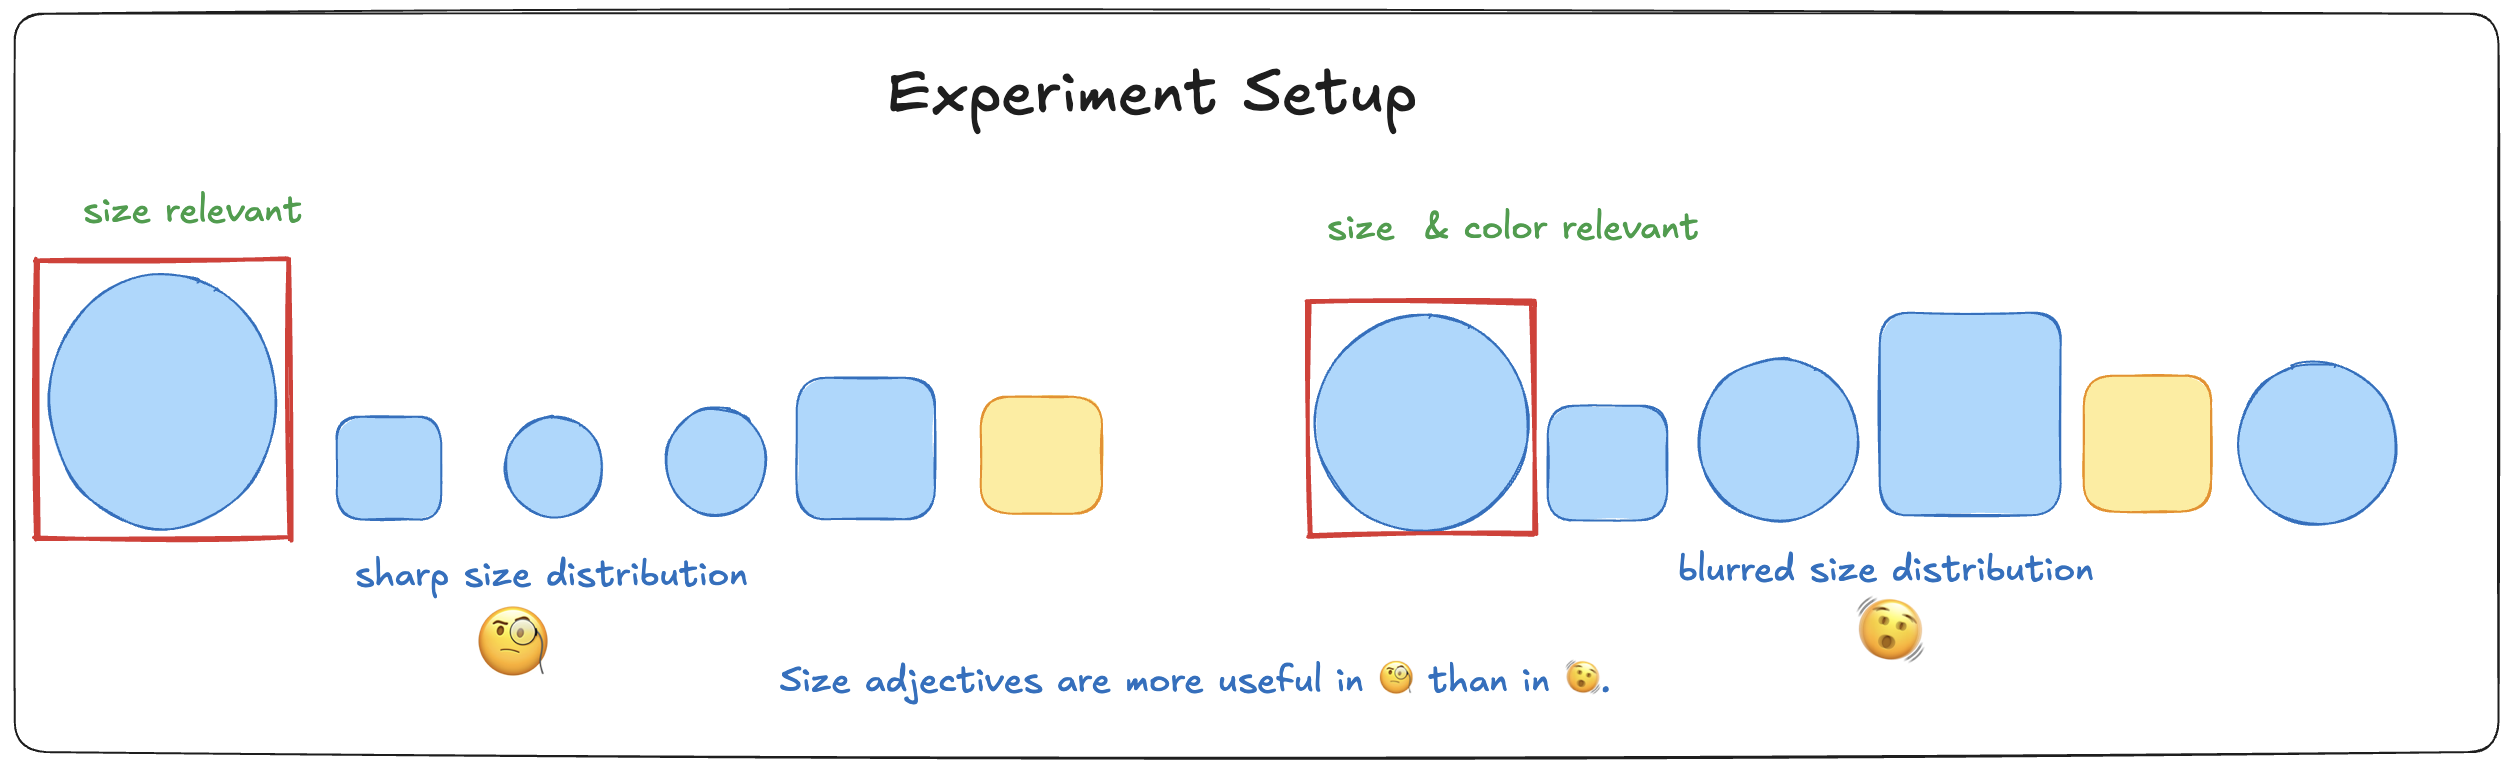
\includegraphics[width=0.7\textwidth]{../../09-presentation/20250710_LMBayes/experiment_item_illustration.png}
  \fbox{\rule{0pt}{4cm}\rule{0.7\textwidth}{0pt}}
  \caption{Illustration of an experiment item (placeholder).  Left panel: a
    sharp-size context; right panel: a blurred-size context.  The referent
    (circled) is the largest, colour-matching, form-matching object.}
  \label{fig:item}
\end{figure}


% -----------------------------------------------------------------------
\subsection{Slider-rating study (Experiment 1)}
\label{sec:exp:slider}
% -----------------------------------------------------------------------

\paragraph{Task.}  Participants rated the \emph{felicity} of each adjective
description on a continuous slider (0--100) for a given context-referent pair.
Ratings were collected for single-adjective (\utter{D}, \utter{C}, \utter{F})
and two-adjective (\utter{DC}, \utter{DF}, \utter{CD}, \etc) descriptions.

\paragraph{Dependent variable.}  Normalised slider ratings, interpreted as
empirical truth values $[\![ u ]\!]_\text{emp}(o, \mathcal{C}) \in [0,1]$.

\paragraph{Key findings.}
\begin{itemize}[leftmargin=*]
  \item Size ratings are markedly lower in the blurred condition than the sharp
    condition, validating the $w_f$ manipulation.
  \item Colour and form ratings are high and stable across conditions.
  \item Ordering interactions: in size-relevant contexts, \utter{DC} is rated
    higher than \utter{CD}; the pattern reverses in colour-relevant contexts.
\end{itemize}

\paragraph{Modelling goal.}
Fit the incremental RSA literal listener to graded slider ratings in order to
estimate $k$, $w_f$, and $\nu$.  These values serve as informative priors for
the production model.

\begin{resbox}{Slider modelling}
  Posterior estimates: $k \approx \todo{X}$, $w_f \approx \todo{X}$ (sharp),
  $w_f \approx \todo{X}$ (blurred), $\nu \approx \todo{X}$.
  \todo{Insert MCMC summary / forest plot here.}
\end{resbox}

\begin{discussbox}{Slider-study discussion}
\begin{itemize}[leftmargin=*]
  \item The slider task confounds \emph{semantic acceptability} with
    \emph{pragmatic felicity}.  How should we interpret the ratings?
  \item Should we run a replication study with a larger sample?
    (A replication dataset is available; results not yet integrated.)
  \item Should $k$ vary by condition or item, or is a single
    population-level value enough?
\end{itemize}
\end{discussbox}


% -----------------------------------------------------------------------
\subsection{Free-production study (Experiment 2)}
\label{sec:exp:production}
% -----------------------------------------------------------------------

\paragraph{Task.}  Participants described the referent object to a hypothetical
listener in as few words as possible, using only the provided adjectives.
Responses were manually annotated into the 15 utterance categories.

\paragraph{Dependent variable.}  Categorical annotation $y_i \in \{1, \ldots, 15\}$
for each trial $i$.

\paragraph{Conditions.}  \todo{$N$ participants, $M$ items, $L$ lists; exact
numbers to be confirmed.}

\paragraph{Key findings.}
\begin{enumerate}[leftmargin=*]
  \item \textbf{Relevant-property effect.}
    Size-first orderings (\utter{D}, \utter{DC}, \utter{DCF}) dominate in
    size-relevant contexts; colour-first (\utter{C}, \utter{CD}) dominate in
    colour-relevant contexts.
  \item \textbf{Sharpness effect.}
    Size adjectives appear more frequently (including over-informatively) in the
    blurred condition than the sharp condition.
  \item \textbf{Single adjective dominance.}
    \utter{D} alone is the modal response across most conditions; multi-word
    utterances are more common when both properties are relevant.
\end{enumerate}

\paragraph{Modelling challenges.}
\begin{itemize}[leftmargin=*]
  \item \emph{Categorical likelihood instability.} Some rare categories have
    near-zero model probability, driving the log-likelihood to $-\infty$.
    Solution: aggregate trials to empirical \emph{soft distributions} per
    condition, and use a Dirichlet likelihood.
  \item \emph{Sparse data per item.} Items with few observations show unreliable
    empirical distributions.  Solution: hierarchical model with item-level
    random effects.
  \item \emph{NUTS + discrete latents.} NUTS requires differentiability; all
    discrete variables (utterance type) must be marginalised.
\end{itemize}

\begin{resbox}{Production modelling}
  \todo{Insert posterior forest plot / predictive check here.}
  Global model: $\alpha \approx \todo{X}$, $\beta \approx \todo{X}$.
  Incremental model: $\mu_k \approx \todo{X}$, $\mu_{w_f} \approx \todo{X}$.
\end{resbox}

\begin{discussbox}{Production-study discussion}
\begin{itemize}[leftmargin=*]
  \item Is the Dirichlet likelihood the right choice, or should we use a
    Multinomial with soft targets?
  \item How do we evaluate model fit beyond visual predictive checks?
    LOO-CV? WAIC?
  \item The production data includes a replication study.  Should the two
    datasets be modelled jointly or separately?
  \item Should the LM prior ($\beta$) be inferred from the data, or is it
    better fixed from corpus statistics?
\end{itemize}
\end{discussbox}

\newpage


% =============================================================================
\section{Simulation}
\label{sec:simulation}
% =============================================================================

\subsection{Goals}
\label{sec:sim:goals}

The simulation has three purposes:
\begin{enumerate}[label=(\arabic*)]
  \item Establish that the incremental speaker \emph{generates} ordering
    preferences, not just accommodates them, across a broad range of contexts.
  \item Map out which parameter region produces a qualitative \emph{big-before-colour}
    preference and compare to a \emph{colour-before-big} region.
  \item Assess robustness: does the ordering preference persist under varying
    context size ($n_\text{obj}$), size-distribution spread ($\sigma_\text{spread}$),
    and perceptual blur ($w_f$)?
\end{enumerate}

\subsection{Design}
\label{sec:sim:design}

\begin{center}
\begin{tabularx}{0.92\textwidth}{lXl}
\toprule
\textbf{Parameter} & \textbf{Values swept} & \textbf{\# levels} \\
\midrule
Speaker model    & Incremental, Global        & 2 \\
$n_\text{obj}$   & 2, 6, 10, 14, 18, 22, 26, 30 & 8 \\
$\sigma_\text{spread}$ & 2.0, 7.75, 15.0 & 3 \\
$\nu$ (colour semantic value) & 0.90, 0.92, 0.94, 0.96, 0.98 & 5 \\
$k$ (threshold)  & 0.10, 0.30, 0.50, 0.70, 0.90 & 5 \\
$w_f$ (perceptual blur) & 0.1, 0.2, 0.3, 0.5, 0.8 & 5 \\
\midrule
\multicolumn{2}{l}{Random context samples per combination} & 1000 \\
\midrule
\multicolumn{2}{l}{\textbf{Total rows}} & \textbf{6,000,000} \\
\bottomrule
\end{tabularx}
\end{center}

Each simulated trial computes communicative success
$p(o_\text{ref} \mid u)$ for two key orderings
(\utter{big blue} $>$ \utter{blue big}) and records which ordering the speaker
model assigns higher probability.

\subsection{Key results}
\label{sec:sim:results}

\todo{Insert simulation plots here -- e.g., proportion of big-first responses
as a function of $k$, $w_f$, and $n_\text{obj}$.}

\begin{resbox}{Simulation findings}
\begin{itemize}[leftmargin=*]
  \item The incremental speaker robustly prefers \utter{D}-first over the
    majority of the parameter space when size is contextually informative.
  \item The threshold parameter $k$ has the largest impact on ordering
    preferences: lower $k$ (higher threshold) reduces size-first preference.
  \item The effect of $n_\text{obj}$ is mediated by $\sigma_\text{spread}$:
    in narrow distributions, larger context size amplifies differences.
  \item The global speaker shows a qualitatively similar but weaker preference,
    suggesting the incremental mechanism is a contributing, not sole, factor.
\end{itemize}
\end{resbox}

\begin{discussbox}{Simulation discussion}
\begin{itemize}[leftmargin=*]
  \item The simulation uses random contexts; should we run it on the actual
    experimental contexts to bridge to the empirical data?
  \item What is the right summary statistic: mean communicative success,
    proportion of trials preferring one ordering, or something else?
  \item Does the simulation yield clear predictions about the replication data?
\end{itemize}
\end{discussbox}

\newpage


% =============================================================================
\section{General Discussion}
\label{sec:discussion}
% =============================================================================

\subsection{Summary}

We have presented an incremental RSA account of adjective ordering preferences
that unifies informativeness-based and subjectivity-based explanations.  The
model is fitted to two complementary datasets (slider ratings and free
production) using NUTS-based Bayesian inference in NumPyro / JAX, and its
qualitative behaviour is validated across a large-scale parameter simulation.

Key claims:
\begin{itemize}[leftmargin=*]
  \item A simple incremental production rule---choose the next adjective
    proportional to its \emph{residual} informativeness---generates ordering
    preferences without a fixed hierarchy.
  \item Perceptual blur ($w_f$) modulates size-adjective usage, explaining the
    sharpness effect.
  \item LM-derived costs provide a grounded utterance prior that is consistent
    with observed single-adjective dominance.
\end{itemize}

\subsection{Open issues for the write-up}

\begin{enumerate}[label=\arabic*., leftmargin=*]
  \item \textbf{Model comparison.}  A formal comparison of global vs.\
    incremental speaker (LOO-CV or Bayes factors) is still outstanding.
  \item \textbf{Replication dataset.}
    The slider-rating replication study needs to be integrated; modelling
    approach not yet finalised.
  \item \textbf{Predictions vs.\ fits.}  Are the parameter values recovered from
    the slider data good priors for the production model?  A formal
    prior-predictive check for the production model is needed.
  \item \textbf{LM prior validation.}  The GPT-derived utterance prior should
    be evaluated against human acceptability judgments.
  \item \textbf{Scope of adjective classes.}  The model currently handles
    D, C, F; extension to other adjective classes (e.g., material, age) is
    not addressed.
  \item \textbf{Individual differences.}  The hierarchical model captures
    item-level variability but not participant-level variability.
  \item \textbf{Write-up structure.}  A tentative section order:
    Introduction $\to$ Background (RSA, adjective ordering) $\to$ Model $\to$
    Experiments $\to$ Results $\to$ Simulation $\to$ General Discussion.
\end{enumerate}

\begin{discussbox}{For the meeting}
\begin{itemize}[leftmargin=*]
  \item What is the right framing for the paper: pragmatics, psycholinguistics,
    or computational linguistics?
  \item Target venue?  \todo{CogSci / Cognition / PLOS ONE / Glossa / ?}
  \item What level of detail should the model section have for the target
    audience?
  \item Figures wish-list: parameter recovery plot, posterior predictive vs.\
    empirical distributions per condition, simulation heatmap.
\end{itemize}
\end{discussbox}


% =============================================================================
\section*{References}
% =============================================================================

\todo{Add references (BibTeX file TBD).  Key citations to include:
Frank \& Goodman (2012), Bergen et al.\ (2016), Scontras et al.\ (2017),
Brehm \& Lam (2019), Piantadosi et al.\ (2012), Pyykkonen et al.\ (ANS semantics).}

\bibliographystyle{apalike}
% \bibliography{references}   % uncomment once references.bib is ready

\end{document}
